
\begin{figure}[H]
  \begin{minipage}[t]{0.45\textwidth}
    \centering
    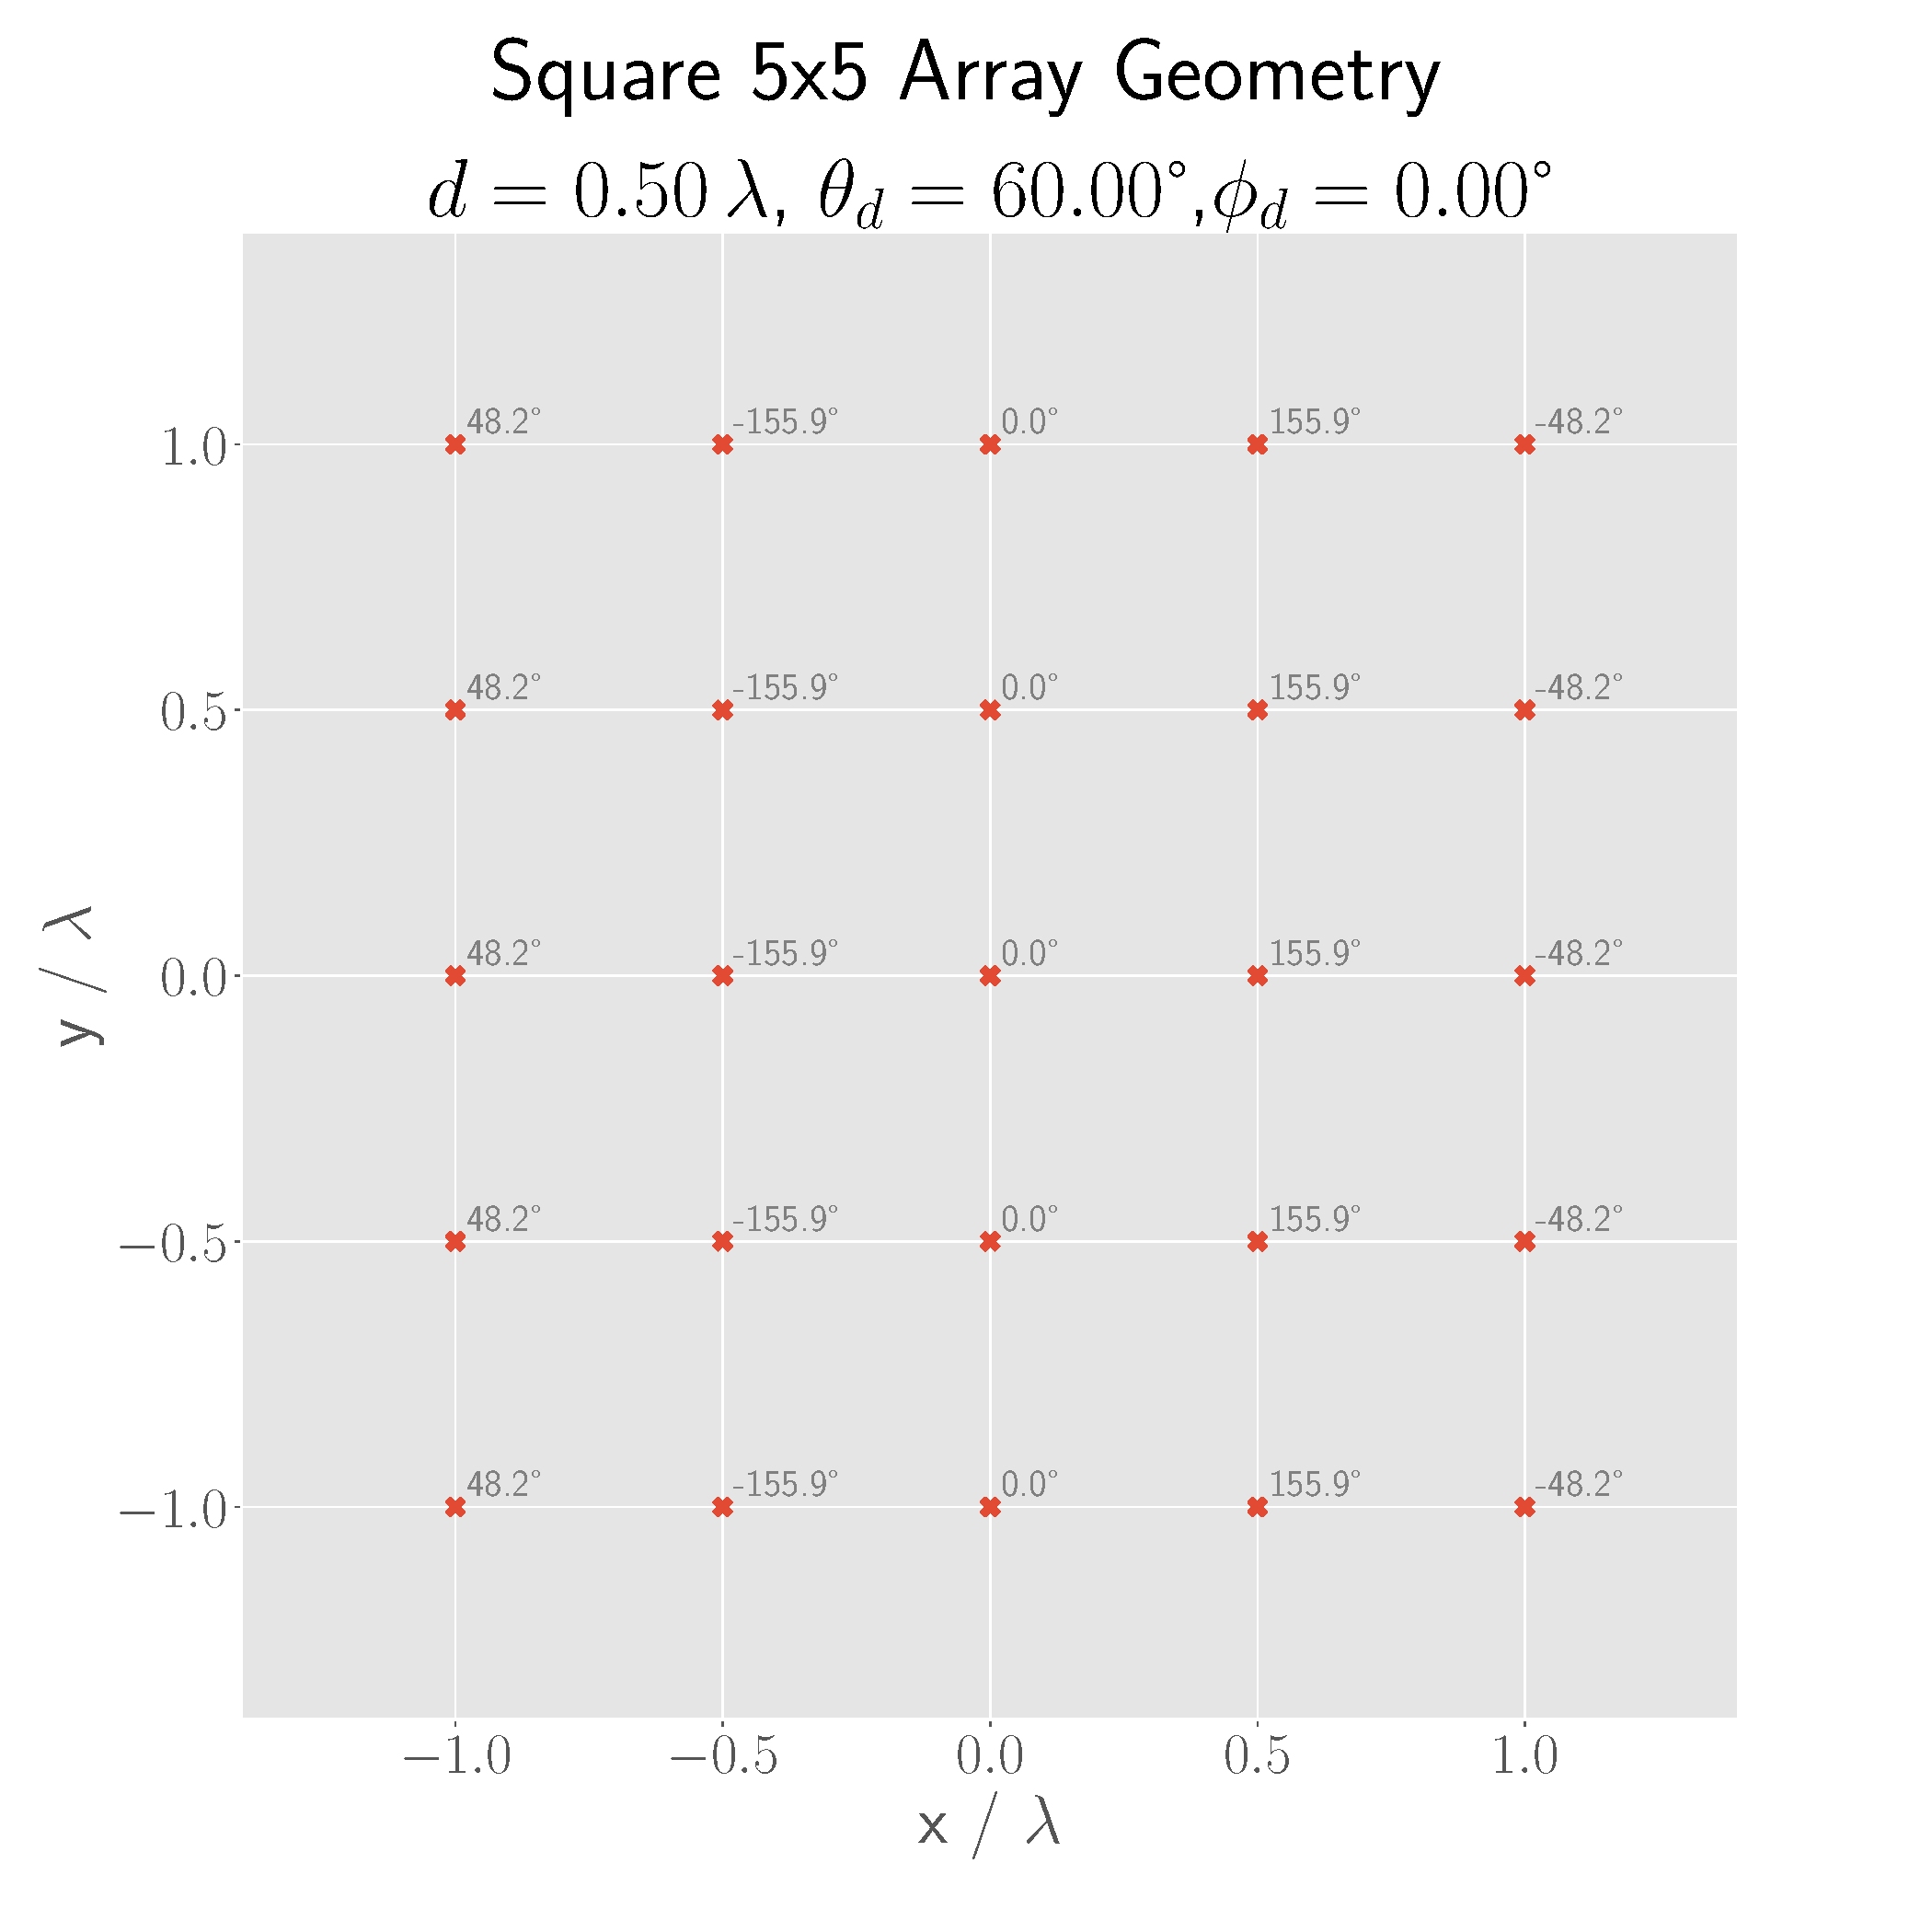
\includegraphics[width=\textwidth]{graphics/task_2/square-0.50-lambda-60.00-theta-0.00-phi-geometry.pdf}
    \caption{Square 5x5 Geometry with steering phases for $0.5\lambda$ spacing.}\label{fig:phase1}
  \end{minipage}\hfill
  \begin{minipage}[t]{0.45\textwidth}
    \centering
    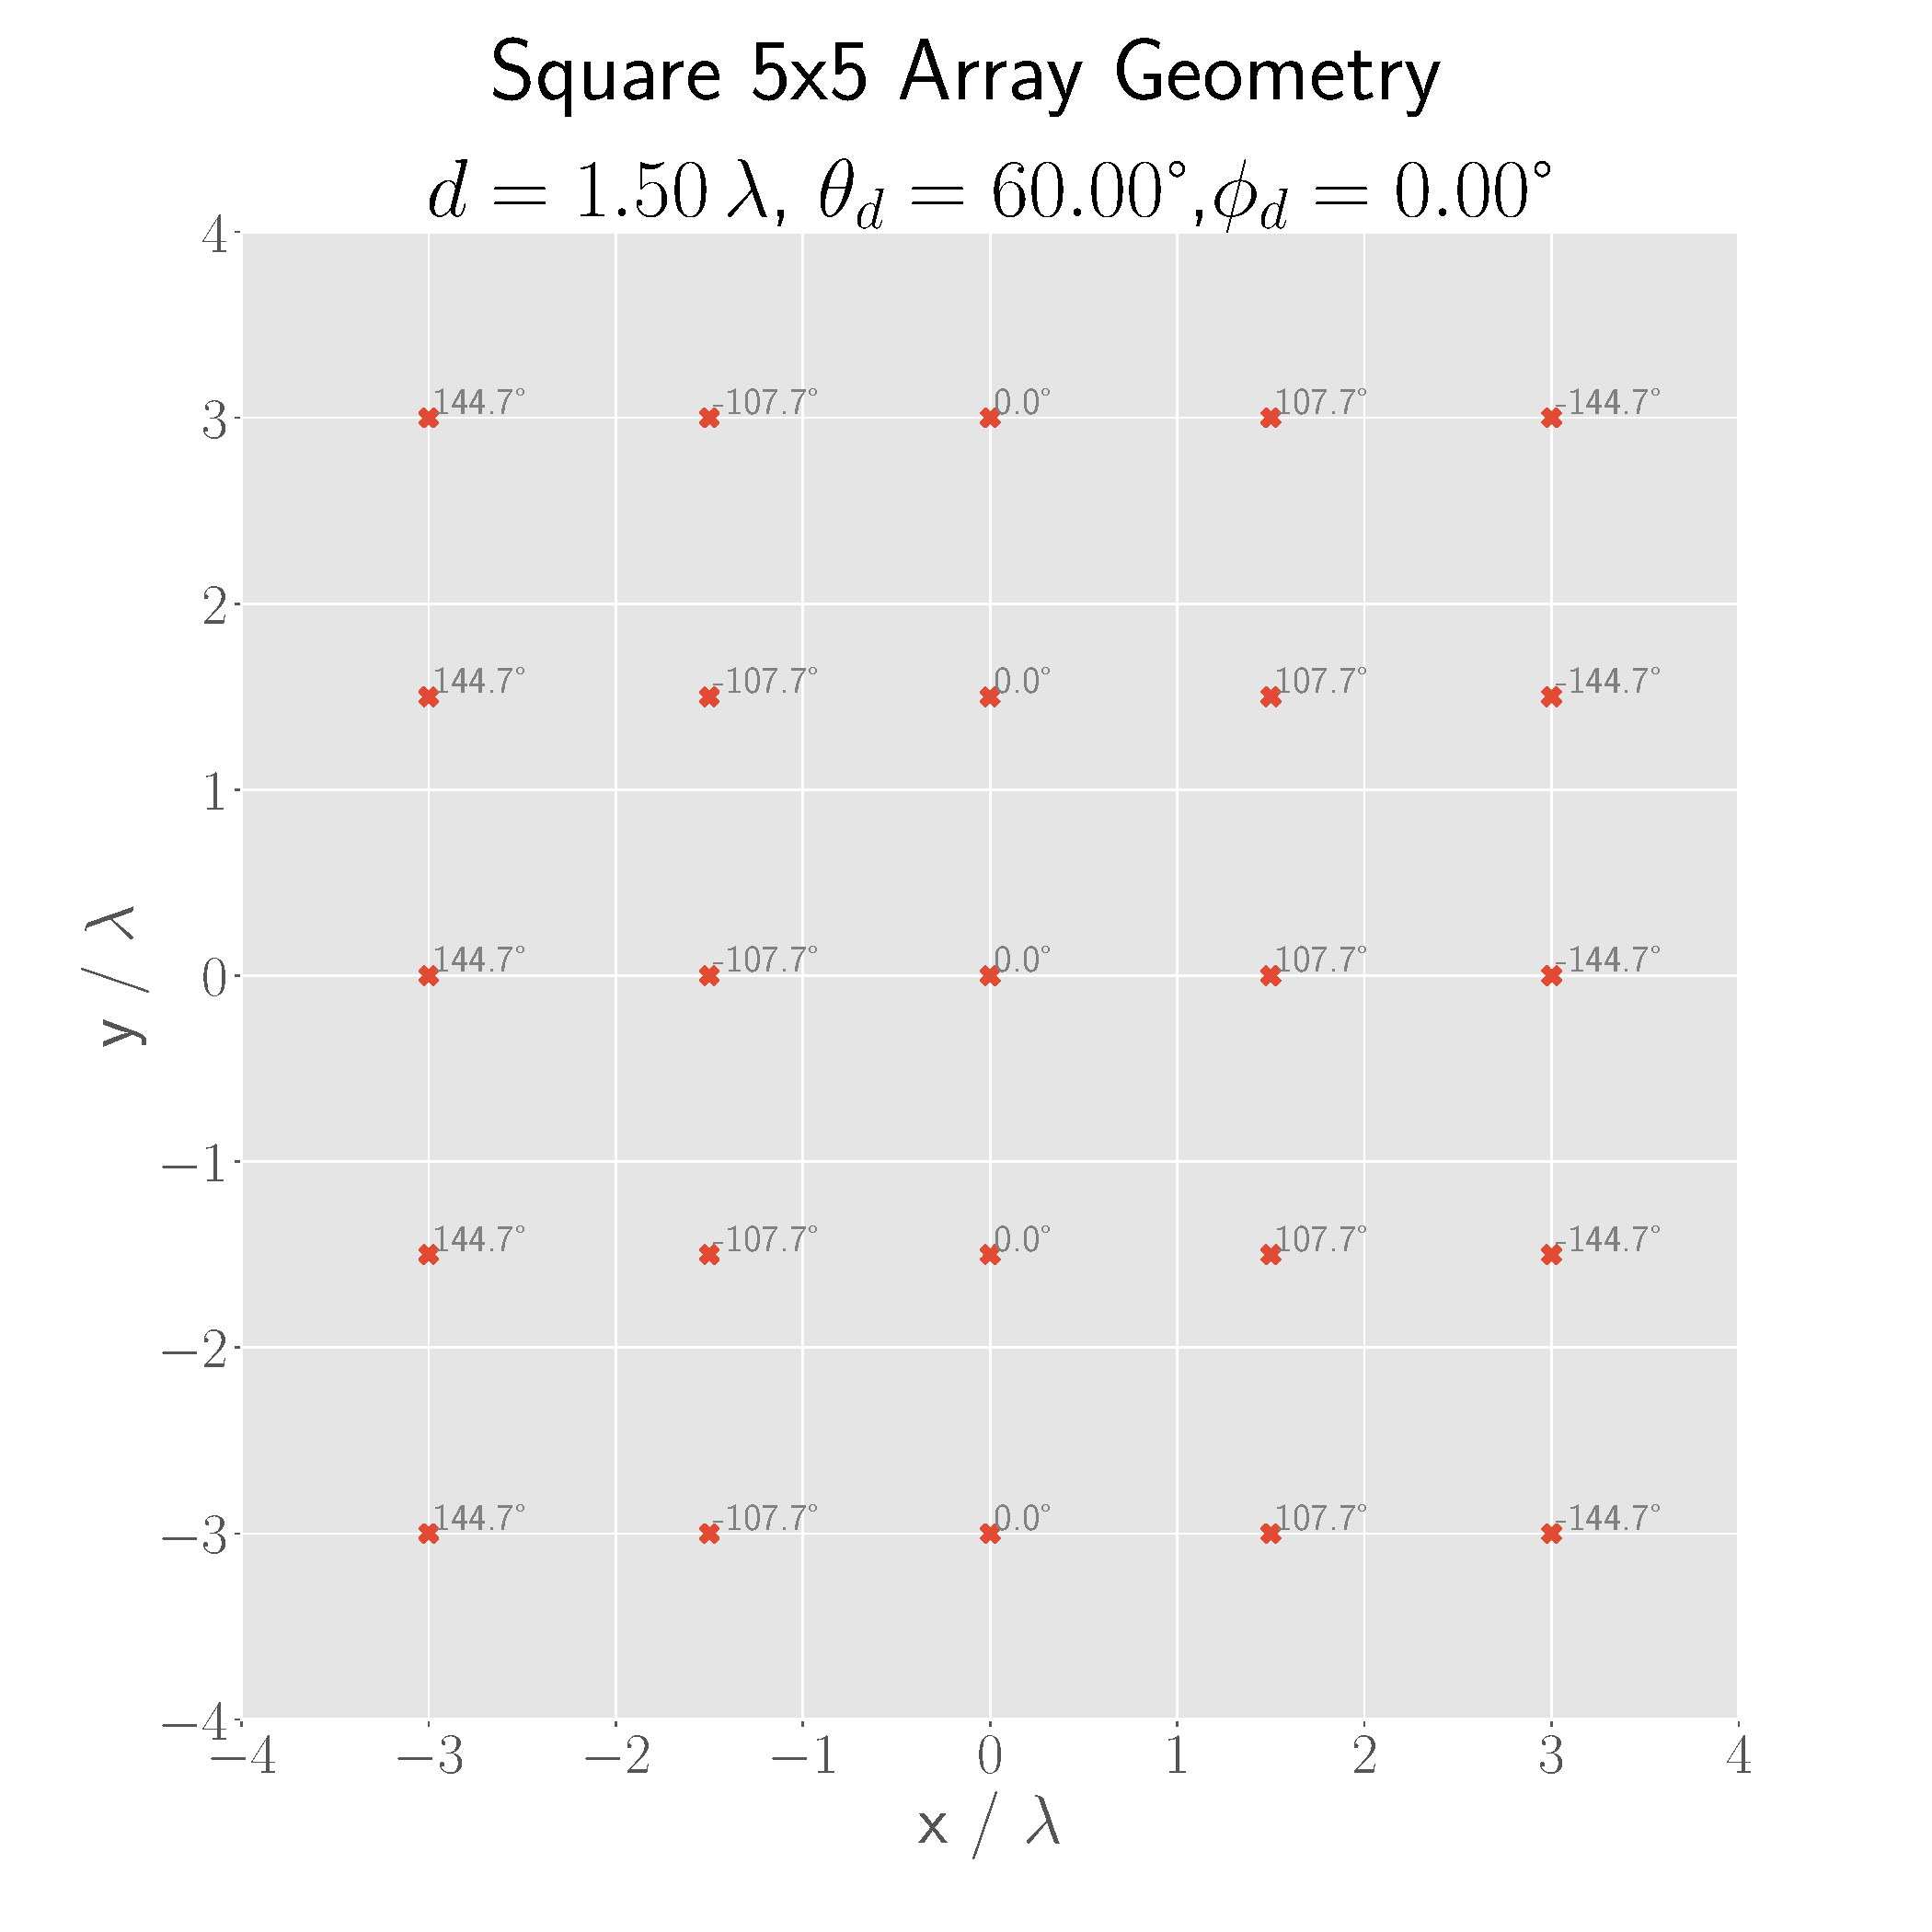
\includegraphics[width=\textwidth]{graphics/task_2/square-1.50-lambda-60.00-theta-0.00-phi-geometry.pdf}
    \caption{Square 5x5 Geometry with steering phases for $1.5\lambda$ spacing.}\label{fig:phase2}
   \end{minipage}
\end{figure}


In figures \ref{fig:phase1} and \ref{fig:phase2}, the array geometries along with the individual steering phases are shown for a target position of $\theta_{d}=60\,\si{\degree}, \phi_{d}=0\,\si{\degree}$. You can see that the phases are constant along the columns since any incident wave from a far-away target will have the same time of arrival for these antennas. Comparing the different spacings, the angle differences in the $d=1.5\lambda$ case are greater, which makes sense since their spacing is larger which results in more time lag.
